% Document settings
\documentclass[a4paper,11pt]{article}

% Packages
  % math formulas
\usepackage{amsmath,amsthm,amssymb}
  % graphics
\usepackage{graphicx}
\usepackage{wrapfig}
  % plots
\usepackage{pgfplots}
  % other
\usepackage[warn]{mathtext}
\usepackage{cmap}
\usepackage[T1,T2A]{fontenc}
\usepackage[utf8]{inputenc}
\usepackage[english,russian]{babel}

% Package settings
%% graphicx
\graphicspath{{Pictures/}}
\DeclareGraphicsExtensions{.pdf,.png,.jpg}
%% pgfplots
\pgfplotsset{width=10cm,compat=1.9}

% Title
\title{Отчет о выполнении работы №1.3.1\\Определение модуля Юнга.}
\author{Воейко Андрей Александрович, Б01-109}
\date{Долгопрудный, 2021}

% Document
\begin{document}
\maketitle
\newpage
\section{Аннотация.}
В работе экспериментально измеряется зависимость между напряжением и деформацией растяжения проволоки. По результатам измерений вычисляется модуль Юнга этой проволоки.
\section{Теоретические сведения.}
Растяжение проволоки соответствует случаю одноосного напряженного состояния, описываемого формулой~\ref{eq1}.
\begin{equation}    \label{eq1}
  \sigma = E \epsilon.
\end{equation}
В работе используется т. н. прибор Лермонтова, изображенный на рисунке~\ref{fig:img1}
\begin{wrapfigure}{r}{0.5\textwidth}
  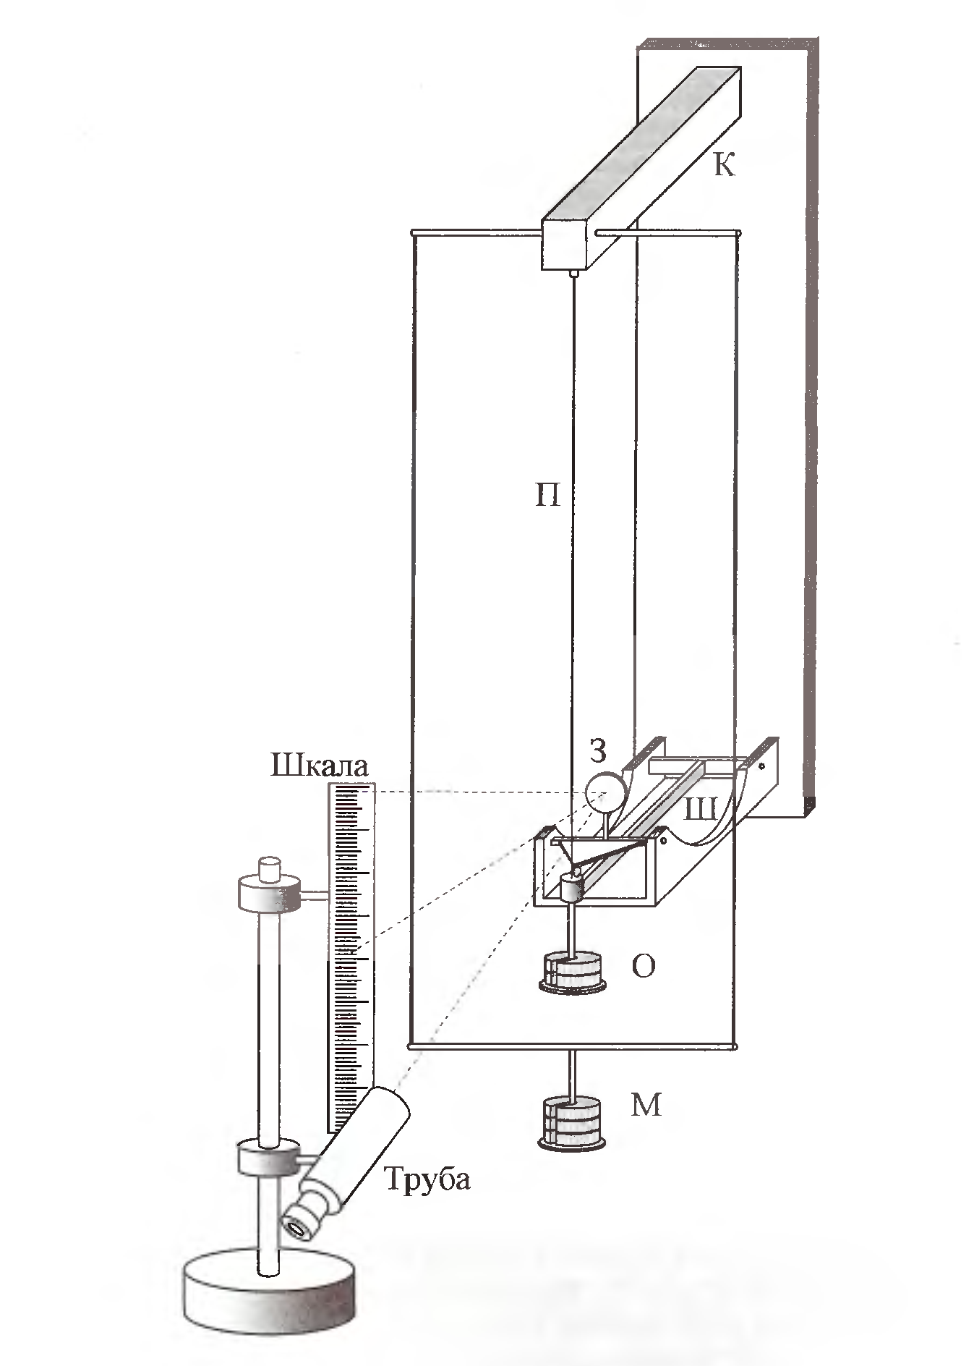
\includegraphics[scale = 0.3]{pic1.png}
  \caption{Прибор Лермонтова.}
  \label{fig:img1}
\end{wrapfigure}
Проволока $П$ одним концом закрепляется в кронштейне $К$, а другим прикреплена к подвешенному через шарнир кронштейну $Ш$. К этому же кронштейну снизу вешаются грузы на площадке $О$. Сами грузы хранятся на площадке $М$, висящей непосредственно на кронштейне $К$, для исключения влияния на результаты эксперимента деформации кронштейна $K$. Также к кронтштейну $Ш$ прикреплено зеркальце, по изменению угла наклона которго можно измерить деформацию проволоки. Угол наклона же вычисляется по изменению отражаемой части шкалы при наблюдении за ней из трубы. Вычисляется он по формуле~\ref{eq2}.
\begin{equation}    \label{eq2}
  \alpha = \frac{\Delta n}{h},
\end{equation}
где $\alpha$ -- это угол наклона зеркальца, $\Delta n$ -- изменение показания шкалы, $h$ -- расстояние от зеркальца до шкалы.
Формула для вычисления удленения проволоки:
\begin{equation}    \label{eq3}
  \Delta l = r \frac{\Delta n}{2h},
\end{equation}
где $\Delta l$ -- изменение длины проволоки, а $r$ -- длина рычажка зеркала.
\section{Оборудование и экспериментальная установка.}
В работе используются:
\begin{itemize}
  \item Прибор Лермонтова.
  \item Набор грузов.
  \item Шкала. Значение -- в сантиметрах, цена деления -- $1\ мм$.
  \item Длина рычажка -- $r = 20\ мм$.
  \item Расстояние от шкалы до зеркальца -- $h = 136,1 \pm 0,1\ см$.
  \item Длина проволоки -- $173,2 \pm 0,1\ см$.
  \item Диаметр проволоки -- $d_{пр} = 0,51\ мм$.
\end{itemize}
\section{Результаты измерений и обработка данных.}
\subsection{Результаты измерений.}
Проведем измерения отражения шкалы в зеркальце, сначала добавляя, а затем убирая грузы с площадки $О$. Повторим измерения трижды. Результаты занесем в таблицу~\ref{table:tab1}.
% Табл. 1 {{{
\begin{table}[h!]
\centering
\begin{tabular}{ ||c|c|c|c|c|c|| }
  \hline
  \multicolumn{3}{||c|}{Серия измерений} & I & II & III \\
  \hline
  Номер верхнего & Масса & Изменение веса & $n_{1}$, & $n_{2}$, & $n_{3}$, \\
  груза $N_{гр}$ & груза $m_{гр}$, $г$ & груза $\Delta P_{гр}$, $г$ & $см$ & $см$ & $см$ \\
  \hline
  $1$ & -- & -- & $8,3 \pm 0,1$ & $8,1 \pm 0,1$ & $8,3 \pm 0,1$ \\
  $2$ & $245,5$ & $+2,41$ & $10,1 \pm 0,1$ & $10,1 \pm 0,1$ & $10,1 \pm 0,1$ \\
  $3$ & $245,6$ & $+2,41$ & $11,9 \pm 0,1$ & $11,9 \pm 0,1$ & $12,0 \pm 0,1$ \\
  $4$ & $244,8$ & $+2,40$ & $13,6 \pm 0,1$ & $13,6 \pm 0,1$ & $13,7 \pm 0,1$ \\
  $5$ & $245,8$ & $+2,41$ & $15,1 \pm 0,1$ & $15,3 \pm 0,1$ & $15,2 \pm 0,1$ \\
  $6$ & $244,9$ & $+2,40$ & $16,8 \pm 0,1$ & $16,8 \pm 0,1$ & $16,9 \pm 0,1$ \\
  $7$ & $245,8$ & $+2,41$ & $18,3 \pm 0,1$ & $18,4 \pm 0,1$ & $18,5 \pm 0,1$ \\
  $8$ & $245,8$ & $+2,41$ & $20,0 \pm 0,1$ & $20,0 \pm 0,1$ & $20,2 \pm 0,1$ \\
  $9$ & $245,7$ & $+2,41$ & $21,6 \pm 0,1$ & $21,6 \pm 0,1$ & $21,7 \pm 0,1$ \\
  $10$ & $245,3$ & $+2,41$ & $23,2 \pm 0,1$ & $23,3 \pm 0,1$ & $23,2 \pm 0,1$ \\
  $9$ & $245,7$ & $-2,41$ & $21,6 \pm 0,1$ & $21,8 \pm 0,1$ & $21,6 \pm 0,1$ \\
  $8$ & $245,8$ & $-2,41$ & $20,1 \pm 0,1$ & $20,2 \pm 0,1$ & $20,2 \pm 0,1$ \\
  $7$ & $245,8$ & $-2,41$ & $18,6 \pm 0,1$ & $18,7 \pm 0,1$ & $18,6 \pm 0,1$ \\
  $6$ & $244,9$ & $-2,41$ & $17,1 \pm 0,1$ & $17,2 \pm 0,1$ & $17,1 \pm 0,1$ \\
  $5$ & $245,8$ & $-2,40$ & $15,3 \pm 0,1$ & $15,5 \pm 0,1$ & $15,5 \pm 0,1$ \\
  $4$ & $244,8$ & $-2,41$ & $13,7 \pm 0,1$ & $13,8 \pm 0,1$ & $13,7 \pm 0,1$ \\
  $3$ & $245,6$ & $-2,40$ & $12,0 \pm 0,1$ & $12,1 \pm 0,1$ & $12,0 \pm 0,1$ \\
  $2$ & $245,5$ & $-2,41$ & $10,2 \pm 0,1$ & $10,2 \pm 0,1$ & $10,3 \pm 0,1$ \\
  \hline
\end{tabular}
\caption{Результаты измерений.}
\label{table:tab1}
\end{table}
% }}}
\subsection{Обработка данных.}
Составим таблицы~\ref{table:tab2}, \ref{table:tab3} и \ref{table:tab4} изменения длины проволоки в первой, второй и третьей сериях измерения соответственно.
% Табл. 2 {{{
\begin{table}[h!]
\centering
\begin{tabular}{ ||c|c|c|c|| }
  \hline
  Номер & Изменение веса & $\Delta n_{1}$, & $\Delta l_{1}$, \\
  шага & груза $\Delta P_{гр}$, $г$ & $см$ & $см$ \\
  \hline
  $1$ & $+2,41$ & $+1,8 \pm 0,2$ & \\
  $2$ & $+2,41$ & $+1,8 \pm 0,2$ & \\
  $3$ & $+2,40$ & $+1,7 \pm 0,2$ & \\
  $4$ & $+2,41$ & $+1,8 \pm 0,2$ & \\
  $5$ & $+2,40$ & $+1,5 \pm 0,2$ & \\
  $6$ & $+2,41$ & $+1,7 \pm 0,2$ & \\
  $7$ & $+2,41$ & $+1,5 \pm 0,2$ & \\
  $8$ & $+2,41$ & $+1,7 \pm 0,2$ & \\
  $9$ & $+2,41$ & $+1,6 \pm 0,2$ & \\
  $10$ & $-2,41$ & $-1,6 \pm 0,2$ & \\
  $11$ & $-2,41$ & $-1,5 \pm 0,2$ & \\
  $12$ & $-2,41$ & $-1,5 \pm 0,2$ & \\
  $13$ & $-2,41$ & $-1,8 \pm 0,2$ & \\
  $14$ & $-2,40$ & $-1,6 \pm 0,2$ & \\
  $15$ & $-2,41$ & $-1,8 \pm 0,2$ & \\
  $16$ & $-2,40$ & $-1,7 \pm 0,2$ & \\
  $17$ & $-2,41$ & $-1,8 \pm 0,2$ & \\
  \hline
\end{tabular}
\caption{Изменения длины проволоки в первой серии измерений.}
\label{table:tab2}
\end{table}
% }}}
% Табл. 3 {{{
\begin{table}[h!]
\centering
\begin{tabular}{ ||c|c|c|c|| }
  \hline
  Номер & Изменение веса & $\Delta n_{1}$, & $\Delta l_{1}$, \\
  шага & груза $\Delta P_{гр}$, $г$ & $см$ & $см$ \\
  \hline
  $1$ & $+2,41$ & $+1,8 \pm 0,2$ & \\
  $2$ & $+2,41$ & $+1,8 \pm 0,2$ & \\
  $3$ & $+2,40$ & $+1,7 \pm 0,2$ & \\
  $4$ & $+2,41$ & $+1,8 \pm 0,2$ & \\
  $5$ & $+2,40$ & $+1,5 \pm 0,2$ & \\
  $6$ & $+2,41$ & $+1,7 \pm 0,2$ & \\
  $7$ & $+2,41$ & $+1,5 \pm 0,2$ & \\
  $8$ & $+2,41$ & $+1,7 \pm 0,2$ & \\
  $9$ & $+2,41$ & $+1,6 \pm 0,2$ & \\
  $10$ & $-2,41$ & $-1,6 \pm 0,2$ & \\
  $11$ & $-2,41$ & $-1,5 \pm 0,2$ & \\
  $12$ & $-2,41$ & $-1,5 \pm 0,2$ & \\
  $13$ & $-2,41$ & $-1,8 \pm 0,2$ & \\
  $14$ & $-2,40$ & $-1,6 \pm 0,2$ & \\
  $15$ & $-2,41$ & $-1,8 \pm 0,2$ & \\
  $16$ & $-2,40$ & $-1,7 \pm 0,2$ & \\
  $17$ & $-2,41$ & $-1,8 \pm 0,2$ & \\
  \hline
\end{tabular}
\caption{Изменения длины проволоки во второй серии измерений.}
\label{table:tab2}
\end{table}
% }}}
% Табл. 4 {{{
\begin{table}[h!]
\centering
\begin{tabular}{ ||c|c|c|c|| }
  \hline
  Номер & Изменение веса & $\Delta n_{1}$, & $\Delta l_{1}$, \\
  шага & груза $\Delta P_{гр}$, $г$ & $см$ & $см$ \\
  \hline
  $1$ & $+2,41$ & $+1,8 \pm 0,2$ & \\
  $2$ & $+2,41$ & $+1,8 \pm 0,2$ & \\
  $3$ & $+2,40$ & $+1,7 \pm 0,2$ & \\
  $4$ & $+2,41$ & $+1,8 \pm 0,2$ & \\
  $5$ & $+2,40$ & $+1,5 \pm 0,2$ & \\
  $6$ & $+2,41$ & $+1,7 \pm 0,2$ & \\
  $7$ & $+2,41$ & $+1,5 \pm 0,2$ & \\
  $8$ & $+2,41$ & $+1,7 \pm 0,2$ & \\
  $9$ & $+2,41$ & $+1,6 \pm 0,2$ & \\
  $10$ & $-2,41$ & $-1,6 \pm 0,2$ & \\
  $11$ & $-2,41$ & $-1,5 \pm 0,2$ & \\
  $12$ & $-2,41$ & $-1,5 \pm 0,2$ & \\
  $13$ & $-2,41$ & $-1,8 \pm 0,2$ & \\
  $14$ & $-2,40$ & $-1,6 \pm 0,2$ & \\
  $15$ & $-2,41$ & $-1,8 \pm 0,2$ & \\
  $16$ & $-2,40$ & $-1,7 \pm 0,2$ & \\
  $17$ & $-2,41$ & $-1,8 \pm 0,2$ & \\
  \hline
\end{tabular}
\caption{Изменения длины проволоки в третьей серии измерений.}
\label{table:tab4}
\end{table}
% }}}
\section{Выводы.}
\end{document}
